\documentclass[11pt]{article}
\usepackage[margin=2.5cm]{geometry}
\usepackage{amsmath, amssymb}
\usepackage{booktabs}
\usepackage{hyperref}
\usepackage{listings}
\usepackage{xcolor}
\usepackage{float}
\usepackage{tikz}
\usetikzlibrary{positioning, arrows.meta, fit, backgrounds}

\lstset{
  language=XML,
  basicstyle=\ttfamily\small,
  keywordstyle=\color{blue},
  stringstyle=\color{red!70!black},
  commentstyle=\color{green!50!black},
  breaklines=true,
  frame=single,
  backgroundcolor=\color{gray!5},
  morekeywords={spec, id, idref, value, network, parameter, weight},
  float=false
}

% Plate diagram styles
\tikzset{
  latent/.style={circle, draw, minimum size=1cm, inner sep=0pt},
  observed/.style={circle, draw, fill=gray!30, minimum size=1cm, inner sep=0pt},
  fixed/.style={circle, draw, double, minimum size=1cm, inner sep=0pt},
  deterministic/.style={circle, draw, double, minimum size=1cm, inner sep=0pt},
  plate/.style={draw, rectangle, rounded corners, inner sep=10pt, dashed},
  arr/.style={-{Stealth[length=6pt]}, thick},
}

\title{CoalPT in BEAST2: Linking the Model to the XML}
\author{}
\date{}

\begin{document}
\maketitle

\noindent This guide maps the mathematical model of the Coalescent with Plasmid Transfer (CoalPT; M\"uller et al.\ 2025, \textit{PLOS Pathogens}, \texttt{10.1371/journal.ppat.1013621}) to the parameters and elements in the BEAST2 XML files used to run it.

\section{The model}

CoalPT models a population of bacteria where each individual carries a chromosome and zero or more plasmids. Going \emph{backward in time}, two types of events can occur:

\begin{itemize}
  \item \textbf{Coalescence}: two lineages merge into a common ancestor.
  \item \textbf{Plasmid transfer}: a plasmid lineage branches off to a different parental lineage (representing a forward-in-time conjugation event).
\end{itemize}

\noindent The result is a phylogenetic \emph{network} $\mathcal{N}$, not a tree. The chromosome tree and each plasmid tree are embedded within this network.

\subsection{Rates}

Let $k$ be the number of extant lineages at a given time. The \textbf{coalescent rate} is
\begin{equation}
  \lambda_{\text{coal}} = \frac{k(k-1)}{2 \, N_e(t)},
\end{equation}
where $N_e(t)$ is the effective population size at time $t$.

For each lineage carrying both the chromosome and $n_p$ plasmids, each plasmid can independently transfer. The \textbf{total plasmid transfer rate} across all lineages is
\begin{equation}
  \lambda_{\text{transfer}} = \sum_{\ell \in \text{lineages}} \sum_{j \in \text{plasmids}(\ell)} \rho_j,
\end{equation}
where $\rho_j$ is the per-lineage transfer rate for plasmid $j$. In the single-plasmid, single-rate case this simplifies to $\lambda_{\text{transfer}} = \rho \cdot m$, where $m$ is the number of lineages carrying the plasmid.

The waiting time to the next event (of either type) is exponentially distributed with rate $\lambda_{\text{coal}} + \lambda_{\text{transfer}}$.

\subsection{Joint posterior}

The posterior density is
\begin{equation}
  P(\mathcal{N}, \boldsymbol{\mu}, N_e, \boldsymbol{\rho} \mid \mathbf{D})
  \propto
  \underbrace{P(\mathbf{D} \mid \mathcal{N}, \boldsymbol{\mu})}_{\text{sequence likelihood}}
  \;\cdot\;
  \underbrace{P(\mathcal{N} \mid N_e, \boldsymbol{\rho})}_{\text{network prior (CoalPT density)}}
  \;\cdot\;
  P(\boldsymbol{\mu}) \; P(N_e) \; P(\boldsymbol{\rho}),
\end{equation}
where $\mathbf{D}$ is the set of sequence alignments (one per segment), $\boldsymbol{\mu}$ collects the substitution model and clock parameters, and $\boldsymbol{\rho}$ is the vector of plasmid transfer rates.

\subsection{Network density (CoalPT density)}

Given a sequence of network events $e_1, e_2, \ldots, e_n$ sorted by time, the log-density of the network is
\begin{equation}
  \log P(\mathcal{N} \mid N_e, \boldsymbol{\rho})
  = \sum_{i} \left[ \underbrace{\log f(e_i)}_{\text{event contribution}} + \underbrace{W(e_{i-1}, e_i)}_{\text{interval contribution}} \right],
\end{equation}
where, for each event $e_i$ at time $t_i$:

\begin{itemize}
  \item If $e_i$ is a \textbf{coalescence}:
    $\log f(e_i) = -\log N_e(t_i)$.

  \item If $e_i$ is a \textbf{plasmid transfer}:
    $\log f(e_i) = \log \rho_j$,
    where $\rho_j$ is the rate for the plasmid being transferred.

  \item If $e_i$ is a \textbf{sample}: no contribution.
\end{itemize}

\noindent The interval contribution between consecutive events is the negative of the total hazard integrated over the interval:
\begin{equation}
  W(e_{i-1}, e_i) = -\lambda_{\text{transfer}}(e_{i-1}) \cdot (t_i - t_{i-1})
                     - \frac{k_{i-1}(k_{i-1} - 1)}{2} \int_{t_{i-1}}^{t_i} \frac{1}{N_e(t)}\, dt,
\end{equation}
where $k_{i-1}$ is the number of lineages and $\lambda_{\text{transfer}}(e_{i-1})$ is the total transfer rate, both evaluated just after event $e_{i-1}$.

\subsection{Sequence likelihood}

Each segment (chromosome or plasmid) has its own embedded tree within the network. The sequence likelihood for segment $s$ is the standard phylogenetic likelihood:
\begin{equation}
  P(\mathbf{D}_s \mid T_s, \boldsymbol{\mu}_s) = \prod_{\text{site } j} \sum_{\text{root state } r} \pi_r \; L_j(r \mid T_s, \boldsymbol{\mu}_s),
\end{equation}
computed via Felsenstein's pruning algorithm. Here $T_s$ is the tree for segment $s$ extracted from $\mathcal{N}$, $\pi_r$ are the base frequencies, and $L_j$ is the conditional site likelihood.

%% ============================================================
\section{Example 1: \texttt{test\_coal.xml} (simulation + inference)}

This XML simulates a network under known parameters, then runs MCMC to recover them. There is no sequence data; only the network density is evaluated.

\subsection{Plate diagram}

\begin{figure}[H]
\centering
\begin{tikzpicture}[node distance=1.5cm]
  % Estimated parameters
  \node[latent] (Ne) {$N_e$};
  \node[latent, right=2.5cm of Ne] (rho) {$\rho$};

  % Network
  \node[latent, below=1.5cm of $(Ne)!0.5!(rho)$] (N) {$\mathcal{N}$};

  % Tip times
  \node[observed, below=1.2cm of N] (tau) {$\boldsymbol{\tau}$};

  % Arrows
  \draw[arr] (Ne) -- (N);
  \draw[arr] (rho) -- (N);
  \draw[arr] (tau) -- (N);

  % Labels
  \node[below=0.3cm of tau, font=\scriptsize, align=center] {tip dates\\(observed)};
\end{tikzpicture}
\caption{Plate diagram for \texttt{test\_coal.xml}. Open circles are latent/estimated variables, shaded circles are observed data. In this example the network $\mathcal{N}$ topology is fixed and only $N_e$ and $\rho$ are estimated via MCMC. No sequence data are used.}
\label{fig:plate-test}
\end{figure}

\subsection{Parameter table}

\begin{table}[H]
\centering
\begin{tabular}{@{} l l l l @{}}
\toprule
\textbf{Model parameter} & \textbf{Symbol} & \textbf{XML id / attribute} & \textbf{Value} \\
\midrule
Effective population size & $N_e$ & \texttt{id="Ne"} & estimated (init: 3) \\
Plasmid transfer rate & $\rho$ & \texttt{id="transfer"} & estimated (init: 3) \\
True $N_e$ (simulation) & $N_e^*$ & \texttt{popSize value="0.5"} & 0.5 (fixed) \\
True $\rho$ (simulation) & $\rho^*$ & \texttt{plasmidTransferRate value="5"} & 5 (fixed) \\
Number of plasmids & $P$ & \texttt{nPlasmids="1"} & 1 \\
\bottomrule
\end{tabular}
\caption{Parameters in \texttt{test\_coal.xml}.}
\end{table}

\subsection{XML--model mapping}

\noindent\begin{minipage}{\linewidth}
\paragraph{Network simulation.}
The \texttt{SimulatedCoalescentWithPlamidsNetwork} element forward-simulates a network under the CoalPT process using the \emph{true} parameter values. The \texttt{nPlasmids="1"} attribute means one chromosome + one plasmid (2 segments). The \texttt{traitSet} with \texttt{date-backward} provides tip sampling times.
\begin{lstlisting}
<!-- The network (simulated under known parameters) -->
<stateNode id="network"
  spec="SimulatedCoalescentWithPlamidsNetwork"
  nPlasmids="1" enableSegmentTreeUpdate="false">
    <populationModel spec="ConstantPopulation">
        <popSize spec="RealParameter" value="0.5"/>
    </populationModel>
    <plasmidTransferRate spec="RealParameter" value="5"/>
    <traitSet ... traitname="date-backward"> ... </traitSet>
</stateNode>
\end{lstlisting}
\end{minipage}

\bigskip
\noindent\begin{minipage}{\linewidth}
\paragraph{Network prior density.}
The \texttt{CoalescentWithPlasmids} element computes $\log P(\mathcal{N} \mid N_e, \rho)$ as described in Section~1.3.
The \texttt{PlasmidNetworkIntervals} element extracts the sorted event list and computes $\lambda_{\text{transfer}}$ at each event.
The parameters \texttt{@transfer} and \texttt{@Ne} are the \emph{estimated} values (distinct from the simulation truth).
\begin{lstlisting}
<!-- Network prior density: P(N | Ne, rho) -->
<distribution id="coalDensity"
  spec="CoalescentWithPlasmids">
    <networkIntervals spec="PlasmidNetworkIntervals"
      network="@network">
        <plasmidTransferRate idref="transfer"/>
    </networkIntervals>
    <populationModel spec="ConstantPopulation">
        <popSize idref="Ne"/>
    </populationModel>
</distribution>
\end{lstlisting}
\end{minipage}

\bigskip
\noindent\begin{minipage}{\linewidth}
\paragraph{Operators.}
Only $\rho$ and $N_e$ are sampled; the network topology is \emph{fixed} (no network operators are included). This tests whether the density computation correctly recovers the simulation parameters.
\begin{lstlisting}
<!-- MCMC operators -->
<operator spec="ScaleOperator" parameter="@transfer" />
<operator spec="ScaleOperator" parameter="@Ne" />
\end{lstlisting}
\end{minipage}

%% ============================================================
\section{Example 2: \texttt{Flexneri\_equal\_rep0.xml} (empirical analysis)}

This XML performs full Bayesian inference on \textit{S.~flexneri} data: chromosome (NC\_004337, 31,711 sites) + one plasmid (NC\_004851, 1,798 sites). Both the network topology and all parameters are estimated.

\subsection{Plate diagram}

\begin{figure}[H]
\centering
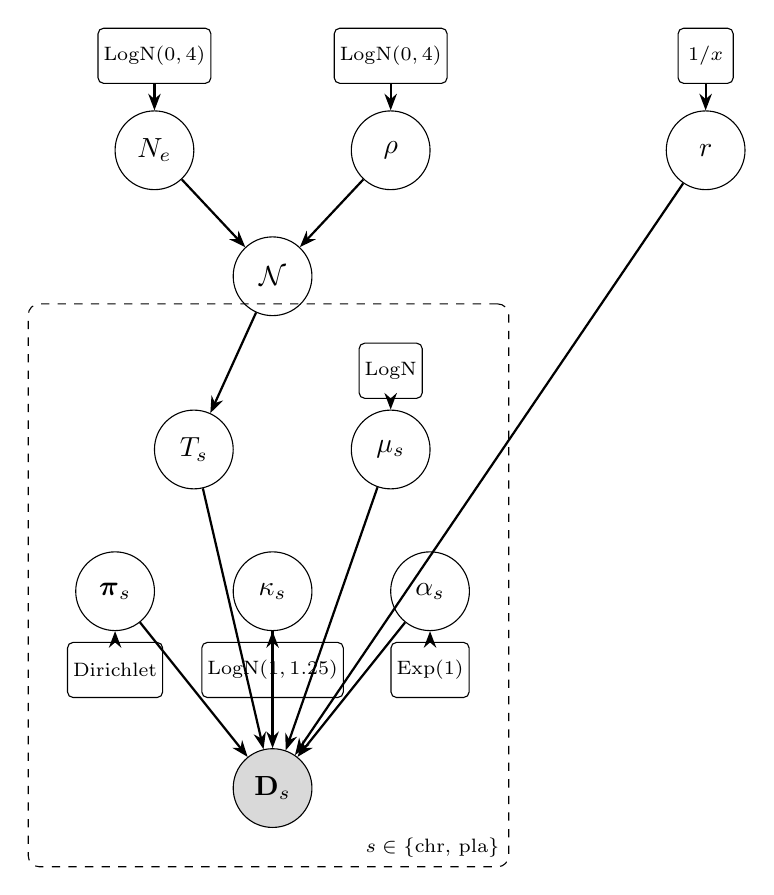
\begin{tikzpicture}[node distance=1.2cm,
  hyperprior/.style={rectangle, draw, rounded corners=2pt, minimum size=0.7cm,
                     inner sep=2pt, font=\scriptsize, fill=white}]

  %% === Use absolute coordinates for clean layout ===

  % Row 1: Hyperpriors for top-level params
  \node[hyperprior] at (0, 0) (pNe) {$\text{LogN}(0,4)$};
  \node[hyperprior] at (3, 0) (prho) {$\text{LogN}(0,4)$};
  \node[hyperprior] at (7, 0) (pr) {$1/x$};

  % Row 2: Top-level parameters
  \node[latent] at (0, -1.2) (Ne) {$N_e$};
  \node[latent] at (3, -1.2) (rho) {$\rho$};
  \node[latent] at (7, -1.2) (r) {$r$};

  \draw[arr] (pNe) -- (Ne);
  \draw[arr] (prho) -- (rho);
  \draw[arr] (pr) -- (r);

  % Row 3: Network
  \node[latent] at (1.5, -2.8) (N) {$\mathcal{N}$};

  \draw[arr] (Ne) -- (N);
  \draw[arr] (rho) -- (N);

  %% === Inside plate ===

  % Row 4: Segment tree + mu with prior
  \node[latent] at (0.5, -5) (Ts) {$T_s$};
  \node[latent] at (3, -5) (mus) {$\mu_s$};
  \node[hyperprior] at (3, -4) (pmu) {$\text{LogN}$};
  \draw[arr] (pmu) -- (mus);
  \draw[arr] (N) -- (Ts);

  % Row 5: pi, kappa, alpha
  \node[latent] at (-0.5, -6.8) (pi) {$\boldsymbol{\pi}_s$};
  \node[latent] at (1.5, -6.8) (kappa) {$\kappa_s$};
  \node[latent] at (3.5, -6.8) (alpha) {$\alpha_s$};

  % Row 6: priors on pi, kappa, alpha
  \node[hyperprior] at (-0.5, -7.8) (ppi) {Dirichlet};
  \node[hyperprior] at (1.5, -7.8) (pkappa) {$\text{LogN}(1, 1.25)$};
  \node[hyperprior] at (3.5, -7.8) (palpha) {$\text{Exp}(1)$};

  \draw[arr] (ppi) -- (pi);
  \draw[arr] (pkappa) -- (kappa);
  \draw[arr] (palpha) -- (alpha);

  % Row 7: Observed data
  \node[observed] at (1.5, -9.3) (Ds) {$\mathbf{D}_s$};

  % Generative arrows into D_s
  \draw[arr] (Ts) -- (Ds);
  \draw[arr] (mus) -- (Ds);
  \draw[arr] (kappa) -- (Ds);
  \draw[arr] (alpha) -- (Ds);
  \draw[arr] (pi) -- (Ds);

  % r arrow into D_s (from outside plate)
  \draw[arr] (r) -- (Ds);

  % Plate box
  \begin{scope}[on background layer]
    \node[plate, fit=(Ts)(mus)(pmu)(kappa)(alpha)(pi)(ppi)(pkappa)(palpha)(Ds),
          inner sep=14pt,
          label={[anchor=south east, font=\scriptsize]south east:$s \in \{\text{chr, pla}\}$}] (plate) {};
  \end{scope}

\end{tikzpicture}
\caption{Plate diagram for \texttt{Flexneri\_equal\_rep0.xml}. Rounded rectangles are fixed prior distributions, open circles are latent/estimated variables, and the shaded circle is observed data. The plate (dashed box) is replicated for each segment $s$ (chromosome and plasmid). The tree $T_s$ is deterministically extracted from the network $\mathcal{N}$. The clock rate $r$ is shared across segments; substitution parameters ($\kappa_s$, $\alpha_s$, $\boldsymbol{\pi}_s$, $\mu_s$) are segment-specific.}
\label{fig:plate-flexneri}
\end{figure}

\subsection{Parameter table}

\begin{table}[H]
\centering
\small
\begin{tabular}{@{} l l l l @{}}
\toprule
\textbf{Model parameter} & \textbf{Symbol} & \textbf{XML id} & \textbf{Initial value} \\
\midrule
Effective population size & $N_e$ & \texttt{Ne} & 100 \\
Plasmid transfer rate & $\rho$ & \texttt{plasmidTransferRate} & 0.1 \\
Clock rate (shared) & $r$ & \texttt{clockRate.c} & 0.0005 \\
Relative mutation rate (chr) & $\mu_{\text{chr}}$ & \texttt{mutationRate.s:NC\_004337} & 1 \\
Relative mutation rate (pla) & $\mu_{\text{pla}}$ & \texttt{mutationRate.s:NC\_004851} & 1 \\
HKY $\kappa$ (chr) & $\kappa_{\text{chr}}$ & \texttt{kappa.s:NC\_004337} & 1.72 \\
HKY $\kappa$ (pla) & $\kappa_{\text{pla}}$ & \texttt{kappa.s:NC\_004851} & 1.53 \\
Gamma shape (chr) & $\alpha_{\text{chr}}$ & \texttt{gammaShape.s:NC\_004337} & 0.50 \\
Gamma shape (pla) & $\alpha_{\text{pla}}$ & \texttt{gammaShape.s:NC\_004851} & 2.73 \\
Base frequencies (chr) & $\boldsymbol{\pi}_{\text{chr}}$ & \texttt{freqParameter.s:NC\_004337} & $(0.25)^4$ \\
Base frequencies (pla) & $\boldsymbol{\pi}_{\text{pla}}$ & \texttt{freqParameter.s:NC\_004851} & $(0.25)^4$ \\
\bottomrule
\end{tabular}
\caption{Parameters in \texttt{Flexneri\_equal\_rep0.xml}. The absolute substitution rate for segment $s$ is $r \cdot \mu_s$.}
\end{table}

\subsection{XML--model mapping}

\noindent\begin{minipage}{\linewidth}
\paragraph{Substitution model.} Each segment uses HKY+$\Gamma_4$ with segment-specific parameters:
\begin{lstlisting}
<siteModel spec="SiteModel" gammaCategoryCount="4"
  shape="@gammaShape.s:NC_004337"
  mutationRate="@mutationRate.s:NC_004337">
    <substModel spec="HKY"
      kappa="@kappa.s:NC_004337">
        <frequencies spec="Frequencies"
          frequencies="@freqParameter.s:NC_004337"/>
    </substModel>
</siteModel>
\end{lstlisting}
\end{minipage}

\bigskip
\noindent\begin{minipage}{\linewidth}
\paragraph{Clock model.} A strict clock with a single shared rate:
\begin{lstlisting}
<branchRateModel
  spec="beast...StrictClockModel"
  clock.rate="@clockRate.c"/>
\end{lstlisting}
A \texttt{DeltaExchangeOperator} constrains the relative rates $\mu_s$ so their weighted mean equals~1:
\begin{lstlisting}
<operator spec="DeltaExchangeOperator" weight="3.0">
    <parameter idref="mutationRate.s:NC_004337"/>
    <parameter idref="mutationRate.s:NC_004851"/>
    <weightvector spec="parameter.IntegerParameter"
      estimate="false">31711 1798</weightvector>
</operator>
\end{lstlisting}
\end{minipage}

\bigskip
\noindent\begin{minipage}{\linewidth}
\paragraph{Network prior.} Same structure as \texttt{test\_coal.xml}:
\begin{lstlisting}
<distribution id="networkPrior"
  spec="coalpt.distribution.CoalescentWithPlasmids">
    <networkIntervals
      spec="coalpt...PlasmidNetworkIntervals"
      network="@network">
        <plasmidTransferRate
          idref="plasmidTransferRate"/>
    </networkIntervals>
    <populationModel spec="ConstantPopulation">
        <popSize idref="Ne"/>
    </populationModel>
</distribution>
\end{lstlisting}
\end{minipage}

\subsection{Priors}

\begin{table}[H]
\centering
\begin{tabular}{@{} l l @{}}
\toprule
\textbf{Parameter} & \textbf{Prior} \\
\midrule
$r$ (clock rate) & $1/x$ (Jeffreys / OneOnX) \\
$N_e$ & LogNormal($M=0$, $S=4$) \\
$\rho$ & LogNormal($M=0$, $S=4$) \\
$\kappa_s$ & LogNormal($M=1$, $S=1.25$) \\
$\alpha_s$ & Exponential(1) \\
$\mu_s$ (relative rate) & LogNormal($M=0.0005$, $S=2$, meanInRealSpace) \\
\bottomrule
\end{tabular}
\caption{Prior distributions in \texttt{Flexneri\_equal\_rep0.xml}.}
\end{table}

\subsection{Network topology operators}

Unlike \texttt{test\_coal.xml}, this analysis includes a full suite of operators that modify the network topology:

\begin{table}[H]
\centering
\small
\begin{tabular}{@{} l l p{6.5cm} @{}}
\toprule
\textbf{Operator class} & \textbf{Weight} & \textbf{Description} \\
\midrule
\texttt{AddRemovePlasmid} & 30 & Adds or removes a plasmid transfer event \\
\texttt{AddRemovePlasmidCoalescent} & 30 & Same, proposing from the coalescent prior \\
\texttt{SubPlasmidNetworkSlide} & 30 & Slides a network node up or down \\
\texttt{UniformNetworkNodeHeight} & 20 & Uniformly resamples internal node heights \\
\texttt{PlasmidNetworkExchange} (wide) & 10 & Wide subtree exchange \\
\texttt{PlasmidNetworkExchange} (narrow) & 5 & Narrow (NNI-like) subtree exchange \\
\texttt{NetworkScaleOperator} & 1 & Scales all node heights \\
\texttt{NetworkScaleOperator} (root) & 1 & Scales only the root height \\
\texttt{NetworkScaleOperator} (up/down) & 1 & Scales network+$N_e$ up, $\rho$+$r$ down \\
\texttt{GibbsOperatorAbovePlasmidRoots} & 3 & Gibbs-samples above plasmid tree roots \\
\bottomrule
\end{tabular}
\caption{Network topology operators in \texttt{Flexneri\_equal\_rep0.xml}.}
\end{table}

\subsection{Inference engine}

This XML uses \texttt{CoupledMCMC} (parallel tempering with 2 chains) rather than standard MCMC, to improve mixing across the complex network space.

%% ============================================================
\section{Segment indexing convention}

CoalPT inherits CoalRe's segment indexing. Segment 0 is the chromosome; segments $1, 2, \ldots, P$ are the plasmids. Each network edge carries a \texttt{BitSet} indicating which segments it transmits. For example, with one plasmid:
\begin{itemize}
  \item \texttt{segments=\{0, 1\}}: edge carries both chromosome and plasmid.
  \item \texttt{segments=\{0\}}: edge carries only the chromosome.
  \item \texttt{segments=\{1\}}: edge carries only the plasmid (arises at a transfer node).
\end{itemize}

\noindent A lineage contributes to the transfer rate only if it carries both the chromosome \emph{and} at least one plasmid (i.e., \texttt{cardinality} $> 1$).

\end{document}
